% 09_pagination_filtering.tex
\chapter{Paginazione e Filtraggio}

La paginazione e il filtraggio sono essenziali per gestire grandi quantità di dati in modo efficiente. Questo capitolo esplora le diverse strategie, best practices e implementazioni.

\section{Introduzione}

\subsection{Perché Paginare}

\begin{tcolorbox}[title=Problemi Senza Paginazione]
\begin{itemize}
\item \textbf{Performance}: Query che ritornano milioni di record sono lente
\item \textbf{Memoria}: Caricare tutti i dati in memoria può causare crash
\item \textbf{Network}: Trasferire grandi dataset consuma banda
\item \textbf{UX}: L'utente non può elaborare migliaia di risultati insieme
\item \textbf{Timeout}: Richieste troppo lunghe possono andare in timeout
\end{itemize}
\end{tcolorbox}

\subsection{Tipi di Paginazione}

\begin{enumerate}
\item \textbf{Offset-based}: Usa offset e limit (tradizionale)
\item \textbf{Cursor-based}: Usa puntatori opachi (efficiente per stream)
\item \textbf{Page-based}: Numerazione pagine (user-friendly)
\item \textbf{Keyset-based}: Usa chiavi ordinabili (efficiente e stabile)
\end{enumerate}

\section{Offset-based Pagination}

\subsection{Concetto}

La paginazione basata su offset usa due parametri:
\begin{itemize}
\item \texttt{limit}: numero di elementi per pagina
\item \texttt{offset}: numero di elementi da saltare
\end{itemize}

\begin{center}
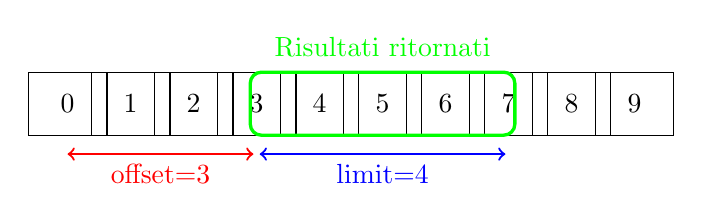
\begin{tikzpicture}[scale=0.8]
  % Database records
  \foreach \i in {0,...,9} {
    \node[draw, minimum width=1cm, minimum height=0.8cm] at (\i, 0) {\i};
  }

  % Offset
  \draw[<->, red, thick] (0, -0.8) -- (2.95, -0.8)
    node[midway, below] {offset=3};

  % Limit
  \draw[<->, blue, thick] (3.05, -0.8) -- (6.95, -0.8)
    node[midway, below] {limit=4};

  % Selected range
  \draw[green, very thick, rounded corners] (2.9, -0.5) rectangle (7.1, 0.5);
  \node[above, green] at (5, 0.6) {Risultati ritornati};
\end{tikzpicture}
\end{center}

\subsection{Esempio Base}

\begin{lstlisting}[language=bash, caption=Request con Offset e Limit]
# Prima pagina (elementi 0-9)
curl "https://api.example.com/users?limit=10&offset=0"

# Seconda pagina (elementi 10-19)
curl "https://api.example.com/users?limit=10&offset=10"

# Terza pagina (elementi 20-29)
curl "https://api.example.com/users?limit=10&offset=20"
\end{lstlisting}

\subsection{Struttura Response}

\begin{lstlisting}[caption=Response Paginata Completa]
{
  "data": [
    {
      "id": 10,
      "name": "Mario Rossi",
      "email": "mario@example.com"
    },
    {
      "id": 11,
      "name": "Laura Bianchi",
      "email": "laura@example.com"
    }
  ],
  "pagination": {
    "total": 1543,
    "count": 10,
    "per_page": 10,
    "current_page": 2,
    "total_pages": 155,
    "links": {
      "first": "https://api.example.com/users?limit=10&offset=0",
      "prev": "https://api.example.com/users?limit=10&offset=0",
      "self": "https://api.example.com/users?limit=10&offset=10",
      "next": "https://api.example.com/users?limit=10&offset=20",
      "last": "https://api.example.com/users?limit=10&offset=1540"
    }
  }
}
\end{lstlisting}

\subsection{Implementazione SQL}

\begin{lstlisting}[language=SQL, caption=Query con LIMIT e OFFSET]
-- PostgreSQL / MySQL
SELECT *
FROM users
ORDER BY id
LIMIT 10 OFFSET 20;

-- SQL Server
SELECT *
FROM users
ORDER BY id
OFFSET 20 ROWS
FETCH NEXT 10 ROWS ONLY;
\end{lstlisting}

\subsection{Implementazione Backend}

\begin{lstlisting}[language=Python, caption=Offset Pagination in Python/Flask]
from flask import Flask, request, jsonify
from sqlalchemy import func

app = Flask(__name__)

@app.route('/api/users')
def get_users():
    # Parametri paginazione
    page = request.args.get('page', 1, type=int)
    per_page = request.args.get('per_page', 10, type=int)

    # Validazione
    per_page = min(per_page, 100)  # Max 100 per pagina
    offset = (page - 1) * per_page

    # Query
    total = db.session.query(func.count(User.id)).scalar()
    users = User.query\
        .order_by(User.id)\
        .limit(per_page)\
        .offset(offset)\
        .all()

    # Calcola pagine totali
    total_pages = (total + per_page - 1) // per_page

    # Costruisci links
    base_url = request.base_url
    links = {
        'self': f"{base_url}?page={page}&per_page={per_page}",
        'first': f"{base_url}?page=1&per_page={per_page}",
        'last': f"{base_url}?page={total_pages}&per_page={per_page}"
    }

    if page > 1:
        links['prev'] = f"{base_url}?page={page-1}&per_page={per_page}"

    if page < total_pages:
        links['next'] = f"{base_url}?page={page+1}&per_page={per_page}"

    return jsonify({
        'data': [user.to_dict() for user in users],
        'pagination': {
            'total': total,
            'count': len(users),
            'per_page': per_page,
            'current_page': page,
            'total_pages': total_pages,
            'links': links
        }
    })
\end{lstlisting}

\subsection{Vantaggi e Svantaggi}

\begin{tcolorbox}[title=Vantaggi]
\begin{itemize}
\item Facile da implementare
\item Supporta salto a pagine specifiche
\item Intuitivo per l'utente
\item Calcolo facile delle pagine totali
\end{itemize}
\end{tcolorbox}

\begin{tcolorbox}[title=Svantaggi, colframe=red!60]
\begin{itemize}
\item \textbf{Performance degradata}: OFFSET alto è lento (deve scansionare record precedenti)
\item \textbf{Inconsistenza}: Se i dati cambiano, elementi possono essere duplicati o saltati
\item \textbf{Non scalabile}: Con milioni di record diventa inutilizzabile
\end{itemize}
\end{tcolorbox}

\section{Cursor-based Pagination}

\subsection{Concetto}

Usa un cursore (puntatore opaco) per identificare la posizione corrente. Ogni pagina include un cursore per la pagina successiva.

\begin{center}
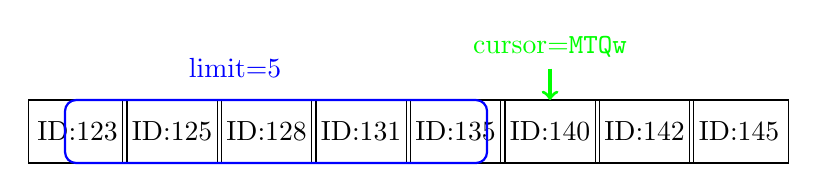
\begin{tikzpicture}[scale=0.8]
  % Records
  \foreach \i/\id in {0/123, 1/125, 2/128, 3/131, 4/135, 5/140, 6/142, 7/145} {
    \node[draw, minimum width=1.2cm, minimum height=0.8cm] at (\i*1.5, 0) {ID:\id};
  }

  % Cursor position
  \draw[->, green, very thick] (5*1.5, 1) -- (5*1.5, 0.5)
    node[above, pos=0] {cursor=\texttt{MTQw}} node[below, pos=1] {};

  % Range
  \draw[blue, thick, rounded corners] (-0.2, -0.5) rectangle (4*1.5+0.5, 0.5);
  \node[above, blue] at (2.5, 0.7) {limit=5};
\end{tikzpicture}
\end{center}

\subsection{Esempio Request}

\begin{lstlisting}[language=bash, caption=Cursor-based Pagination]
# Prima pagina
curl "https://api.example.com/users?limit=10"

# Pagina successiva (usa cursor dalla response)
curl "https://api.example.com/users?limit=10&cursor=eyJpZCI6MTB9"

# Cursore e' opaco (es. Base64 di {"id": 10})
echo "eyJpZCI6MTB9" | base64 -d
# Output: {"id":10}
\end{lstlisting}

\subsection{Struttura Response}

\begin{lstlisting}[caption=Response con Cursori]
{
  "data": [
    {"id": 1, "name": "User 1"},
    {"id": 2, "name": "User 2"},
    {"id": 5, "name": "User 5"},
    {"id": 7, "name": "User 7"},
    {"id": 10, "name": "User 10"}
  ],
  "paging": {
    "cursors": {
      "before": "eyJpZCI6MX0=",
      "after": "eyJpZCI6MTB9"
    },
    "next": "https://api.example.com/users?limit=10&cursor=eyJpZCI6MTB9",
    "has_next": true
  }
}
\end{lstlisting}

\subsection{Implementazione}

\begin{lstlisting}[language=Python, caption=Cursor Pagination Implementation]
import base64
import json
from flask import Flask, request, jsonify

def encode_cursor(data):
    """Codifica dati in cursore opaco"""
    json_str = json.dumps(data)
    return base64.b64encode(json_str.encode()).decode()

def decode_cursor(cursor):
    """Decodifica cursore"""
    try:
        json_str = base64.b64decode(cursor.encode()).decode()
        return json.loads(json_str)
    except:
        return None

@app.route('/api/users')
def get_users_cursor():
    limit = request.args.get('limit', 10, type=int)
    limit = min(limit, 100)  # Max 100

    cursor = request.args.get('cursor')

    # Costruisci query
    query = User.query.order_by(User.id)

    # Applica cursore se presente
    if cursor:
        cursor_data = decode_cursor(cursor)
        if cursor_data and 'id' in cursor_data:
            query = query.filter(User.id > cursor_data['id'])

    # Fetch limit + 1 per sapere se ci sono piu' risultati
    users = query.limit(limit + 1).all()

    # Check se ci sono piu' pagine
    has_next = len(users) > limit
    if has_next:
        users = users[:limit]

    # Costruisci response
    data = [user.to_dict() for user in users]

    response = {'data': data}

    if users:
        # Cursori
        first_cursor = encode_cursor({'id': users[0].id - 1})
        last_cursor = encode_cursor({'id': users[-1].id})

        # Next URL
        next_url = None
        if has_next:
            next_url = f"{request.base_url}?limit={limit}&cursor={last_cursor}"

        response['paging'] = {
            'cursors': {
                'before': first_cursor,
                'after': last_cursor
            },
            'next': next_url,
            'has_next': has_next
        }

    return jsonify(response)
\end{lstlisting}

\subsection{Query SQL con Cursor}

\begin{lstlisting}[language=SQL, caption=Cursor-based SQL Query]
-- Assumendo cursor = {"id": 100}
SELECT *
FROM users
WHERE id > 100
ORDER BY id
LIMIT 10;

-- Per cursore con timestamp
SELECT *
FROM posts
WHERE created_at < '2023-11-13 12:00:00'
ORDER BY created_at DESC
LIMIT 20;
\end{lstlisting}

\subsection{Vantaggi e Svantaggi}

\begin{tcolorbox}[title=Vantaggi]
\begin{itemize}
\item Performance costante (usa indici)
\item Nessun problema con dati che cambiano
\item Scalabile a grandi dataset
\item Ideale per stream infiniti
\end{itemize}
\end{tcolorbox}

\begin{tcolorbox}[title=Svantaggi, colframe=red!60]
\begin{itemize}
\item Non puoi saltare a pagine arbitrarie
\item Nessun conteggio totale
\item Più complesso da implementare
\item Richiede campo ordinabile univoco
\end{itemize}
\end{tcolorbox}

\section{Page-based Pagination}

\subsection{Concetto}

Simile a offset ma usa numero di pagina invece di offset.

\begin{lstlisting}[language=bash, caption=Page Number Pagination]
# Pagina 1
curl "https://api.example.com/users?page=1&per_page=10"

# Pagina 2
curl "https://api.example.com/users?page=2&per_page=10"

# Equivale a: offset = (page - 1) * per_page
\end{lstlisting}

\subsection{Link Headers (RFC 5988)}

\begin{lstlisting}[caption=Paginazione con Link Headers]
HTTP/1.1 200 OK
Content-Type: application/json
Link: <https://api.example.com/users?page=1&per_page=10>; rel="first",
      <https://api.example.com/users?page=3&per_page=10>; rel="prev",
      <https://api.example.com/users?page=5&per_page=10>; rel="next",
      <https://api.example.com/users?page=155&per_page=10>; rel="last"

{
  "data": [...]
}
\end{lstlisting>

\subsection{Implementazione Link Headers}

\begin{lstlisting}[language=Python, caption=Generazione Link Headers]
from flask import Response
import json

def generate_link_header(base_url, page, per_page, total_pages):
    """Genera Link header per paginazione"""
    links = []

    # First
    links.append(f'<{base_url}?page=1&per_page={per_page}>; rel="first"')

    # Prev
    if page > 1:
        links.append(
            f'<{base_url}?page={page-1}&per_page={per_page}>; rel="prev"'
        )

    # Next
    if page < total_pages:
        links.append(
            f'<{base_url}?page={page+1}&per_page={per_page}>; rel="next"'
        )

    # Last
    links.append(
        f'<{base_url}?page={total_pages}&per_page={per_page}>; rel="last"'
    )

    return ', '.join(links)

@app.route('/api/users')
def get_users_with_link_header():
    page = request.args.get('page', 1, type=int)
    per_page = request.args.get('per_page', 10, type=int)

    # Query (vedi implementazione precedente)
    # ...

    # Crea response
    response_data = json.dumps({'data': data})
    response = Response(response_data, mimetype='application/json')

    # Aggiungi Link header
    link_header = generate_link_header(
        request.base_url, page, per_page, total_pages
    )
    response.headers['Link'] = link_header

    return response
\end{lstlisting}

\section{Keyset Pagination}

\subsection{Concetto}

Usa valori della chiave di ordinamento invece di offset.

\begin{lstlisting}[language=bash, caption=Keyset Pagination]
# Prima richiesta
curl "https://api.example.com/posts?limit=10&sort=created_at"

# Richieste successive usano l'ultimo valore
curl "https://api.example.com/posts?limit=10&sort=created_at&after=2023-11-13T12:00:00Z"
\end{lstlisting}

\subsection{Implementazione}

\begin{lstlisting}[language=SQL, caption=Keyset SQL Query]
-- Prima pagina
SELECT id, title, created_at
FROM posts
ORDER BY created_at DESC, id DESC
LIMIT 10;

-- Pagine successive (assumendo ultimo created_at = '2023-11-13 12:00:00', id = 1543)
SELECT id, title, created_at
FROM posts
WHERE (created_at, id) < ('2023-11-13 12:00:00', 1543)
ORDER BY created_at DESC, id DESC
LIMIT 10;
\end{lstlisting}

\begin{lstlisting}[language=Python, caption=Keyset Pagination in Python]
@app.route('/api/posts')
def get_posts_keyset():
    limit = request.args.get('limit', 10, type=int)
    after_time = request.args.get('after_time')
    after_id = request.args.get('after_id', type=int)

    query = Post.query.order_by(
        Post.created_at.desc(),
        Post.id.desc()
    )

    # Applica keyset
    if after_time and after_id:
        query = query.filter(
            db.or_(
                Post.created_at < after_time,
                db.and_(
                    Post.created_at == after_time,
                    Post.id < after_id
                )
            )
        )

    posts = query.limit(limit + 1).all()

    has_next = len(posts) > limit
    if has_next:
        posts = posts[:limit]

    # Response
    data = [post.to_dict() for post in posts]

    response = {'data': data}

    if posts and has_next:
        last_post = posts[-1]
        next_url = (
            f"{request.base_url}?limit={limit}"
            f"&after_time={last_post.created_at.isoformat()}"
            f"&after_id={last_post.id}"
        )
        response['next'] = next_url

    return jsonify(response)
\end{lstlisting}

\section{Filtraggio}

\subsection{Query Parameters per Filtri}

\begin{lstlisting}[language=bash, caption=Esempi di Filtraggio]
# Filtro semplice
curl "https://api.example.com/users?status=active"

# Filtri multipli
curl "https://api.example.com/users?status=active&role=admin"

# Filtro con range
curl "https://api.example.com/products?price_min=10&price_max=100"

# Filtro con data
curl "https://api.example.com/posts?created_after=2023-01-01"

# Filtro con pattern matching
curl "https://api.example.com/users?email_like=@gmail.com"
\end{lstlisting}

\subsection{Operatori di Filtro}

\begin{table}[h]
\centering
\begin{tabular}{|l|l|p{7cm}|}
\hline
\textbf{Operatore} & \textbf{Query Param} & \textbf{Esempio} \\ \hline
Uguale & \texttt{field=value} & \texttt{status=active} \\ \hline
Non uguale & \texttt{field[ne]=value} & \texttt{status[ne]=deleted} \\ \hline
Maggiore & \texttt{field[gt]=value} & \texttt{age[gt]=18} \\ \hline
Maggiore/uguale & \texttt{field[gte]=value} & \texttt{price[gte]=100} \\ \hline
Minore & \texttt{field[lt]=value} & \texttt{stock[lt]=10} \\ \hline
Minore/uguale & \texttt{field[lte]=value} & \texttt{created[lte]=2023-12-31} \\ \hline
In lista & \texttt{field[in]=v1,v2} & \texttt{status[in]=active,pending} \\ \hline
Like & \texttt{field[like]=pattern} & \texttt{name[like]=\%john\%} \\ \hline
\end{tabular}
\caption{Operatori di Filtro Comuni}
\end{table}

\subsection{Implementazione Filtri Dinamici}

\begin{lstlisting}[language=Python, caption=Sistema di Filtri Flessibile]
from sqlalchemy import and_, or_

class FilterBuilder:
    """Costruisce filtri dinamici da query parameters"""

    # Mappa operatori a funzioni SQLAlchemy
    OPERATORS = {
        'eq': lambda field, value: field == value,
        'ne': lambda field, value: field != value,
        'gt': lambda field, value: field > value,
        'gte': lambda field, value: field >= value,
        'lt': lambda field, value: field < value,
        'lte': lambda field, value: field <= value,
        'in': lambda field, value: field.in_(value.split(',')),
        'like': lambda field, value: field.like(value),
        'ilike': lambda field, value: field.ilike(value),
    }

    # Campi filtrabili (whitelist per sicurezza)
    FILTERABLE_FIELDS = {
        'User': ['status', 'role', 'email', 'created_at'],
        'Product': ['category', 'price', 'in_stock']
    }

    @classmethod
    def build_filters(cls, model, query_params):
        """Costruisce filtri da query parameters"""
        filters = []
        model_name = model.__name__

        for param, value in query_params.items():
            # Parse parametro: field[operator] o field
            if '[' in param:
                field_name, operator = param.replace(']', '').split('[')
            else:
                field_name = param
                operator = 'eq'

            # Validazione campo
            if field_name not in cls.FILTERABLE_FIELDS.get(model_name, []):
                continue

            # Ottieni campo del model
            field = getattr(model, field_name, None)
            if not field:
                continue

            # Applica operatore
            if operator in cls.OPERATORS:
                filter_func = cls.OPERATORS[operator]
                filters.append(filter_func(field, value))

        return filters

@app.route('/api/users')
def get_filtered_users():
    # Costruisci filtri da query params
    filters = FilterBuilder.build_filters(User, request.args)

    # Applica filtri
    query = User.query
    if filters:
        query = query.filter(and_(*filters))

    # Paginazione
    page = request.args.get('page', 1, type=int)
    per_page = request.args.get('per_page', 10, type=int)

    # Execute
    users = query.paginate(page=page, per_page=per_page)

    return jsonify({
        'data': [user.to_dict() for user in users.items],
        'pagination': {
            'page': page,
            'per_page': per_page,
            'total': users.total,
            'pages': users.pages
        }
    })
\end{lstlisting}

\subsection{Esempio Completo con Filtri}

\begin{lstlisting}[language=bash, caption=Query Complessa]
curl -G "https://api.example.com/products" \
  --data-urlencode "category=electronics" \
  --data-urlencode "price[gte]=100" \
  --data-urlencode "price[lte]=500" \
  --data-urlencode "in_stock=true" \
  --data-urlencode "brand[in]=Sony,Samsung,LG" \
  --data-urlencode "name[like]=%TV%" \
  --data-urlencode "sort=-price,name" \
  --data-urlencode "page=2" \
  --data-urlencode "per_page=20"
\end{lstlisting}

\section{Ordinamento}

\subsection{Query Parameters per Sort}

\begin{lstlisting}[language=bash, caption=Parametri di Ordinamento]
# Ordinamento singolo (ascendente)
curl "https://api.example.com/users?sort=name"

# Ordinamento discendente (prefisso -)
curl "https://api.example.com/users?sort=-created_at"

# Ordinamento multiplo
curl "https://api.example.com/users?sort=status,-created_at,name"
\end{lstlisting}

\subsection{Implementazione Sort}

\begin{lstlisting}[language=Python, caption=Dynamic Sorting]
class SortBuilder:
    """Costruisce ordinamenti dinamici"""

    # Whitelist campi ordinabili
    SORTABLE_FIELDS = {
        'User': ['id', 'name', 'email', 'created_at', 'status'],
        'Product': ['id', 'name', 'price', 'created_at']
    }

    @classmethod
    def build_sort(cls, model, sort_param):
        """
        Costruisce ordinamento da parametro sort
        Formato: campo1,-campo2,campo3
        Prefisso - indica discendente
        """
        if not sort_param:
            return []

        model_name = model.__name__
        sort_fields = []

        for field_expr in sort_param.split(','):
            # Determina direzione
            if field_expr.startswith('-'):
                field_name = field_expr[1:]
                direction = 'desc'
            else:
                field_name = field_expr
                direction = 'asc'

            # Validazione
            if field_name not in cls.SORTABLE_FIELDS.get(model_name, []):
                continue

            # Ottieni campo
            field = getattr(model, field_name, None)
            if not field:
                continue

            # Aggiungi ordinamento
            if direction == 'desc':
                sort_fields.append(field.desc())
            else:
                sort_fields.append(field.asc())

        return sort_fields

@app.route('/api/users')
def get_sorted_users():
    # Ordinamento
    sort_param = request.args.get('sort')
    sort_fields = SortBuilder.build_sort(User, sort_param)

    # Query
    query = User.query
    if sort_fields:
        query = query.order_by(*sort_fields)
    else:
        query = query.order_by(User.id)  # Default

    # ... paginazione ...
\end{lstlisting}

\section{Field Selection (Sparse Fieldsets)}

\subsection{Concetto}

Permette al client di specificare quali campi vuole ricevere.

\begin{lstlisting}[language=bash, caption=Field Selection]
# Solo alcuni campi
curl "https://api.example.com/users?fields=id,name,email"

# Campi per risorse correlate
curl "https://api.example.com/posts?fields[posts]=id,title&fields[author]=name,email"
\end{lstlisting}

\subsection{Implementazione}

\begin{lstlisting}[language=Python, caption=Dynamic Field Selection]
def select_fields(obj, fields):
    """Seleziona solo i campi richiesti"""
    if not fields:
        return obj.to_dict()

    field_list = fields.split(',')
    result = {}

    for field in field_list:
        if hasattr(obj, field):
            value = getattr(obj, field)
            # Converti datetime, etc
            if isinstance(value, datetime):
                value = value.isoformat()
            result[field] = value

    return result

@app.route('/api/users')
def get_users_sparse():
    fields = request.args.get('fields')

    users = User.query.limit(10).all()

    data = [select_fields(user, fields) for user in users]

    return jsonify({'data': data})
\end{lstlisting}

\section{HATEOAS e Link Navigation}

\subsection{Hypermedia Controls}

\begin{lstlisting}[caption=Response con HATEOAS Links]
{
  "data": [
    {
      "id": 1,
      "name": "Product 1",
      "price": 99.99,
      "_links": {
        "self": {
          "href": "https://api.example.com/products/1"
        },
        "category": {
          "href": "https://api.example.com/categories/electronics"
        },
        "reviews": {
          "href": "https://api.example.com/products/1/reviews"
        }
      }
    }
  ],
  "_links": {
    "self": {
      "href": "https://api.example.com/products?page=2"
    },
    "first": {
      "href": "https://api.example.com/products?page=1"
    },
    "prev": {
      "href": "https://api.example.com/products?page=1"
    },
    "next": {
      "href": "https://api.example.com/products?page=3"
    },
    "last": {
      "href": "https://api.example.com/products?page=50"
    }
  },
  "_meta": {
    "total_items": 500,
    "item_count": 10,
    "items_per_page": 10,
    "total_pages": 50,
    "current_page": 2
  }
}
\end{lstlisting}

\subsection{HAL (Hypertext Application Language)}

\begin{lstlisting}[caption=HAL Format Response]
{
  "_links": {
    "self": {"href": "/orders/523"},
    "warehouse": {"href": "/warehouses/56"},
    "invoice": {"href": "/invoices/873"}
  },
  "currency": "USD",
  "status": "shipped",
  "total": 10.20,
  "_embedded": {
    "items": [
      {
        "_links": {"self": {"href": "/products/123"}},
        "name": "Widget",
        "price": 5.10,
        "quantity": 2
      }
    ]
  }
}
\end{lstlisting}

\section{Best Practices}

\subsection{Limiti Ragionevoli}

\begin{lstlisting}[language=Python, caption=Validazione Parametri Paginazione]
def validate_pagination_params(page, per_page):
    """Valida e normalizza parametri paginazione"""

    # Limiti di sicurezza
    MAX_PER_PAGE = 100
    DEFAULT_PER_PAGE = 10

    # Normalizza
    page = max(1, page)
    per_page = min(max(1, per_page), MAX_PER_PAGE)

    # Warn se al massimo
    if per_page >= MAX_PER_PAGE:
        logger.warning(
            f"Client requested max pagination size: {per_page}"
        )

    return page, per_page
\end{lstlisting}

\subsection{Caching}

\begin{lstlisting}[caption=Cache Headers per Risposte Paginate]
HTTP/1.1 200 OK
Content-Type: application/json
Cache-Control: public, max-age=60
ETag: "33a64df551425fcc55e4d42a148795d9f25f89d4"
Vary: Accept, Accept-Encoding

{
  "data": [...]
}
\end{lstlisting}

\subsection{Documentazione Parametri}

\begin{lstlisting}[caption=OpenAPI Schema per Paginazione]
openapi: 3.0.0
paths:
  /users:
    get:
      summary: List users
      parameters:
        - name: page
          in: query
          description: Page number (1-indexed)
          schema:
            type: integer
            minimum: 1
            default: 1

        - name: per_page
          in: query
          description: Items per page
          schema:
            type: integer
            minimum: 1
            maximum: 100
            default: 10

        - name: sort
          in: query
          description: |
            Sort fields (comma-separated).
            Prefix with - for descending.
            Example: -created_at,name
          schema:
            type: string
          example: "-created_at,name"

        - name: status
          in: query
          description: Filter by status
          schema:
            type: string
            enum: [active, inactive, pending]

        - name: created_after
          in: query
          description: Filter by creation date
          schema:
            type: string
            format: date-time

      responses:
        '200':
          description: Paginated users list
          content:
            application/json:
              schema:
                type: object
                properties:
                  data:
                    type: array
                    items:
                      $ref: '#/components/schemas/User'
                  pagination:
                    type: object
                    properties:
                      total:
                        type: integer
                      page:
                        type: integer
                      per_page:
                        type: integer
                      pages:
                        type: integer
                      links:
                        type: object
                        properties:
                          first:
                            type: string
                            format: uri
                          prev:
                            type: string
                            format: uri
                          self:
                            type: string
                            format: uri
                          next:
                            type: string
                            format: uri
                          last:
                            type: string
                            format: uri
\end{lstlisting}

\section{Esempi Completi}

\subsection{Client JavaScript}

\begin{lstlisting}[language=JavaScript, caption=Fetch Paginato in JavaScript]
class PaginatedAPI {
  constructor(baseUrl, token) {
    this.baseUrl = baseUrl;
    this.token = token;
  }

  async fetchPage(endpoint, params = {}) {
    const queryString = new URLSearchParams(params).toString();
    const url = `${this.baseUrl}${endpoint}?${queryString}`;

    const response = await fetch(url, {
      headers: {
        'Authorization': `Bearer ${this.token}`,
        'Accept': 'application/json'
      }
    });

    if (!response.ok) {
      throw new Error(`HTTP ${response.status}`);
    }

    return response.json();
  }

  async *fetchAllPages(endpoint, params = {}) {
    let page = 1;
    let hasMore = true;

    while (hasMore) {
      const data = await this.fetchPage(endpoint, {
        ...params,
        page,
        per_page: 100
      });

      yield data.data;

      hasMore = data.pagination.links.next !== null;
      page++;
    }
  }

  async fetchAll(endpoint, params = {}) {
    const allData = [];

    for await (const pageData of this.fetchAllPages(endpoint, params)) {
      allData.push(...pageData);
    }

    return allData;
  }
}

// Utilizzo
const api = new PaginatedAPI('https://api.example.com', 'token123');

// Fetch singola pagina
const page1 = await api.fetchPage('/users', {page: 1, per_page: 20});

// Fetch tutte le pagine (generator)
for await (const users of api.fetchAllPages('/users', {status: 'active'})) {
  console.log(`Fetched ${users.length} users`);
  processUsers(users);
}

// Fetch tutti i dati
const allUsers = await api.fetchAll('/users');
\end{lstlisting}

\subsection{Script Bash Completo}

\begin{lstlisting}[language=bash, caption=Paginazione in Bash]
#!/bin/bash

API_URL="https://api.example.com"
TOKEN="your-api-token"

fetch_all_pages() {
  local endpoint=$1
  local page=1
  local total_fetched=0

  while true; do
    echo "Fetching page $page..."

    response=$(curl -s \
      -H "Authorization: Bearer $TOKEN" \
      "$API_URL$endpoint?page=$page&per_page=100")

    # Estrai dati
    data=$(echo "$response" | jq '.data')
    count=$(echo "$data" | jq 'length')

    if [ "$count" -eq 0 ]; then
      echo "No more data"
      break
    fi

    # Processa dati
    echo "$data" | jq -c '.[]' | while read item; do
      # Processa ogni item
      echo "$item"
    done

    total_fetched=$((total_fetched + count))
    echo "Total fetched: $total_fetched"

    # Check se ci sono altre pagine
    has_next=$(echo "$response" | jq -r '.pagination.links.next // empty')

    if [ -z "$has_next" ]; then
      echo "Reached last page"
      break
    fi

    page=$((page + 1))
  done
}

# Utilizzo
fetch_all_pages "/users"
\end{lstlisting}

\section{Riepilogo}

\begin{table}[h]
\centering
\small
\begin{tabular}{|l|l|l|l|}
\hline
\textbf{Strategia} & \textbf{Pro} & \textbf{Contro} & \textbf{Quando Usarla} \\ \hline
Offset & Semplice, pagine numerate & Lento con offset alto & Dataset piccoli/medi \\ \hline
Cursor & Performance costante & Non salta pagine & Stream, feed, dataset grandi \\ \hline
Page & User-friendly & Come offset & UI con navigazione pagine \\ \hline
Keyset & Veloce, stabile & Complesso & Dataset grandi ordinati \\ \hline
\end{tabular}
\caption{Confronto Strategie di Paginazione}
\end{table}

\begin{tcolorbox}[title=Checklist Paginazione/Filtraggio]
\begin{itemize}
\item[$\square$] Implementa limiti massimi (max 100-1000 item per pagina)
\item[$\square$] Fornisci link navigazionali (next, prev, first, last)
\item[$\square$] Documenta parametri e formati chiaramente
\item[$\square$] Valida e sanitizza tutti i parametri
\item[$\square$] Usa indici database per campi filtrabili/ordinabili
\item[$\square$] Implementa field selection per ridurre payload
\item[$\square$] Considera cache per richieste comuni
\item[$\square$] Fornisci metadati (total, pages, etc)
\end{itemize}
\end{tcolorbox}
